\documentclass[a4paper,14pt]{extarticle}

\usepackage[a4paper,top=20mm,bottom=20mm,left=30mm,right=10mm]{geometry}
\usepackage[T1,T2A]{fontenc}
\usepackage[utf8]{inputenc}
\usepackage[russian]{babel}
\usepackage{indentfirst}
\usepackage{titlesec}
\usepackage{graphicx}
\usepackage{verbatim}
\usepackage{fancyvrb}
\usepackage{nicematrix}

\renewcommand{\baselinestretch}{1.3}
\titleformat{\section}{\normalsize\bfseries}{\thesection}{1em}{}
\titleformat{\subsection}{\normalsize\bfseries}{\thesection}{1em}{}
\setlength{\parindent}{12.5mm}

\begin{document}

  \newpage\thispagestyle{empty}
  \begin{center}
    \MakeUppercase{
      Министерство науки и высшего образования Российской Федерации\\
      Федеральное государственное бюджетное образовательное учреждение высшего образования\\
      <<Вятский Государственный Университет>>\\
    }
    Институт математики и информационных систем\\
    Факультет автоматики и вычислительной техники\\
    Кафедра электронных вычислительных машин
  \end{center}
  \vfill
  
  \begin{center}
    \textbf{Работа с множествами}\\
    Отчёт по лабораторной работе №1\\
    по дисциплине\\
    <<Дискретная математика>>\\
    Вариант 5
  \end{center}
  \vfill
  
  \noindent
  \begin{tabular}{ll}
    Выполнил студент гр. ИВТб-1301-05-00 \hspace{5mm} &
    \rule[-1mm]{25mm}{0.10mm}\,/Макаров С.А./\\
    
    Руководитель преподаватель & \rule[-1mm]{25mm}{0.10mm}\,/Пахарева И.В./\\
  \end{tabular}
  
  \vfill
  \begin{center}
    Киров 2025
  \end{center}
  
  \newpage
  \section*{Цель}
  Цель лабораторной работы: изучение основ теории множеств, базовых операций над ними, разработка приложения на языке Паскаль согласно заданию.
  
  \section*{Задание}
  Требуется реализовать программу для выполнения заданных операций над множествами:
  \begin{enumerate}
    \item Программа должна позволять вводить до десяти с однолитеральными именами (A, B, C и т.д.) за счёт использования с жёстко заданным синтаксисом <имя множества> = <элемент 1>, <элемент 2>, .... Множество может включать в себя до десяти элементов.
    
    \item Программа должна позволять выполнять заданные операции над введёнными множествами за счёт использования строки с жёстко заданным синтаксисом, с выводом результата в качестве работы.
    
    \item В случае некорректного введения строки в пунктах 1 и 2 должно появляться информационное сообщение об ошибке.
  \end{enumerate}
  
  Данные для выполнения задания:\\
  $\cup$ -- объединение множеств\\
  $\cap$ -- пересечение множеств\\
  / -- разность множеств\\
  $\triangle$ -- симметричная разность множеств\\
  N -- множество натуральных чисел\\
  Z -- множество целых чисел\\
  Q -- множество рациональных чисел\\
  I -- множество иррациональных чисел\\
  R -- множество действительных чисел\\
  рус. -- множество букв русского алфавита\\
  лат. -- множество букв латинского алфавита\\
  
  \noindent Таблица 1 -- Вариант задания\\
  \begin{NiceTabularX}{\textwidth}{cXXXXXccc}[hvlines, cell-space-top-limit=1mm]
    вар./множ. & \centering A & \centering B & \centering C & \centering D & \centering E & X & Y & K \\
    
    5 & \centering R & \centering Q & \centering N & \centering лат. & \centering рус. & A$\cap$B$\cap$C & E$\triangle$D & X$\cap$Y
  \end{NiceTabularX}\\
  
  В таблице 1 представлены множества в соответствии с вариантом.
  
  \section*{Решение}
  Для решением задач разработана схема алгоритма, представленная на рисунках 1, 2, 3, 4.
  \begin{figure}[h]
    \centering
    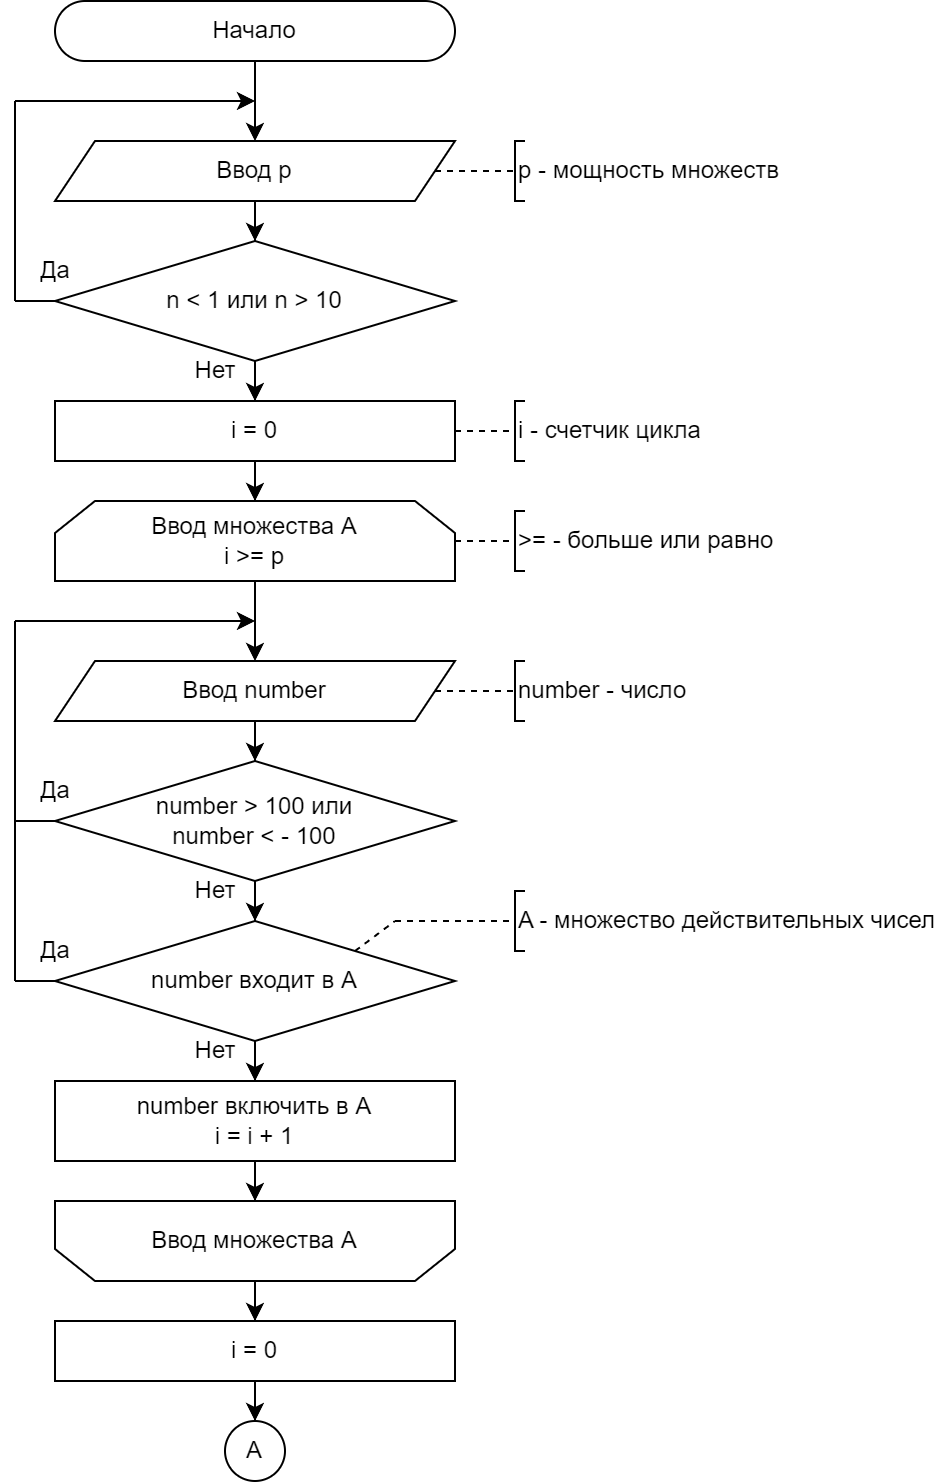
\includegraphics[width=0.6\linewidth]{images/s-1}
  \end{figure}
  \begin{center}
    Рисунок 1 – Схема алгоритма программы
  \end{center}
  
  \pagebreak
  \begin{figure}[h]
    \centering
    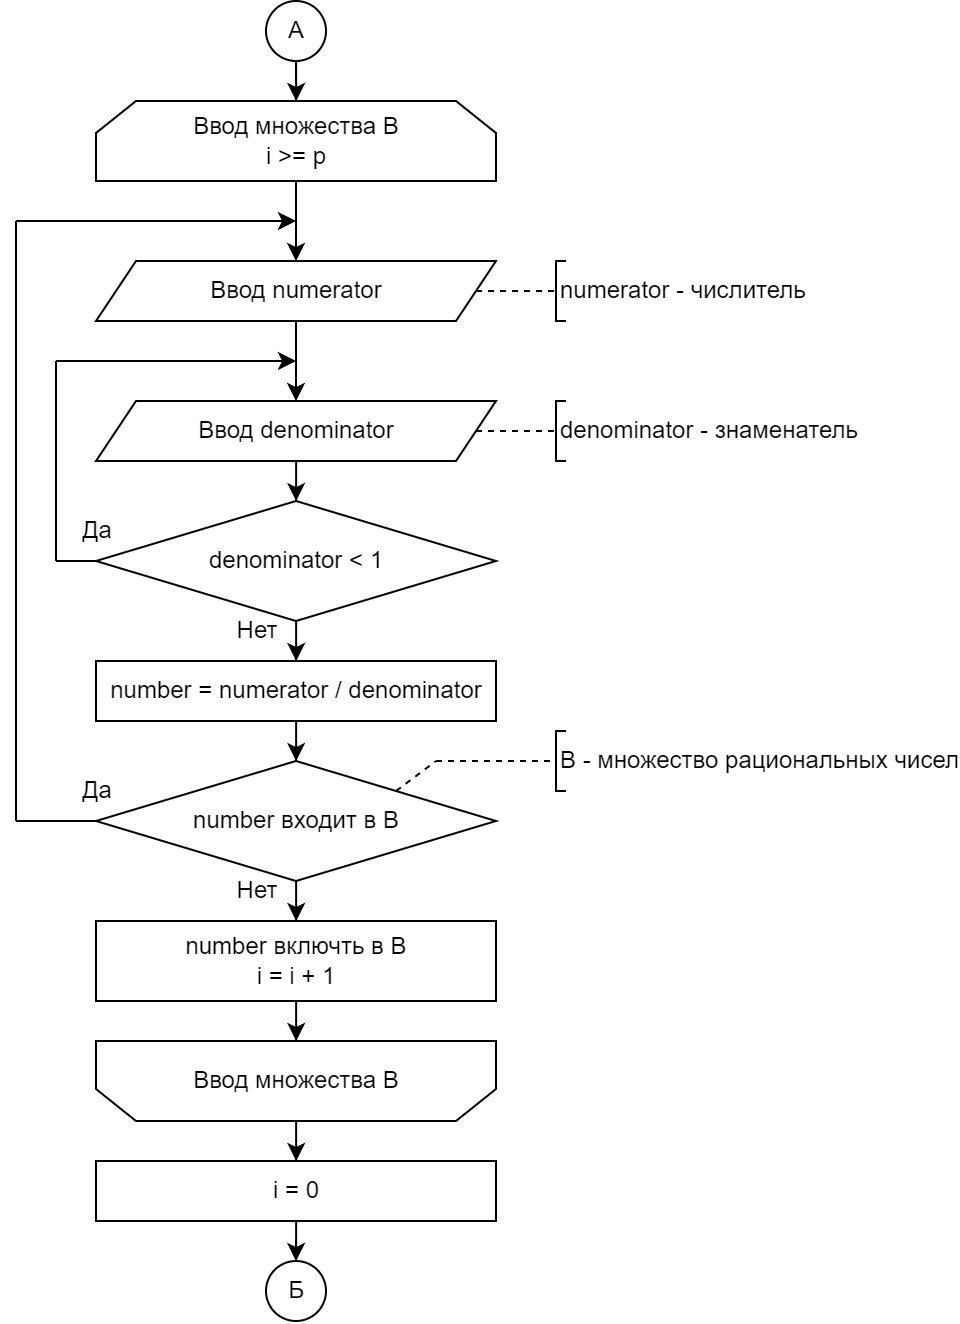
\includegraphics[width=0.7\linewidth]{images/s-2}
  \end{figure}
  \begin{center}
    Рисунок 2 – Продолжение схемы алгоритма программы
  \end{center}
  
  \pagebreak
  \begin{figure}[h]
    \centering
    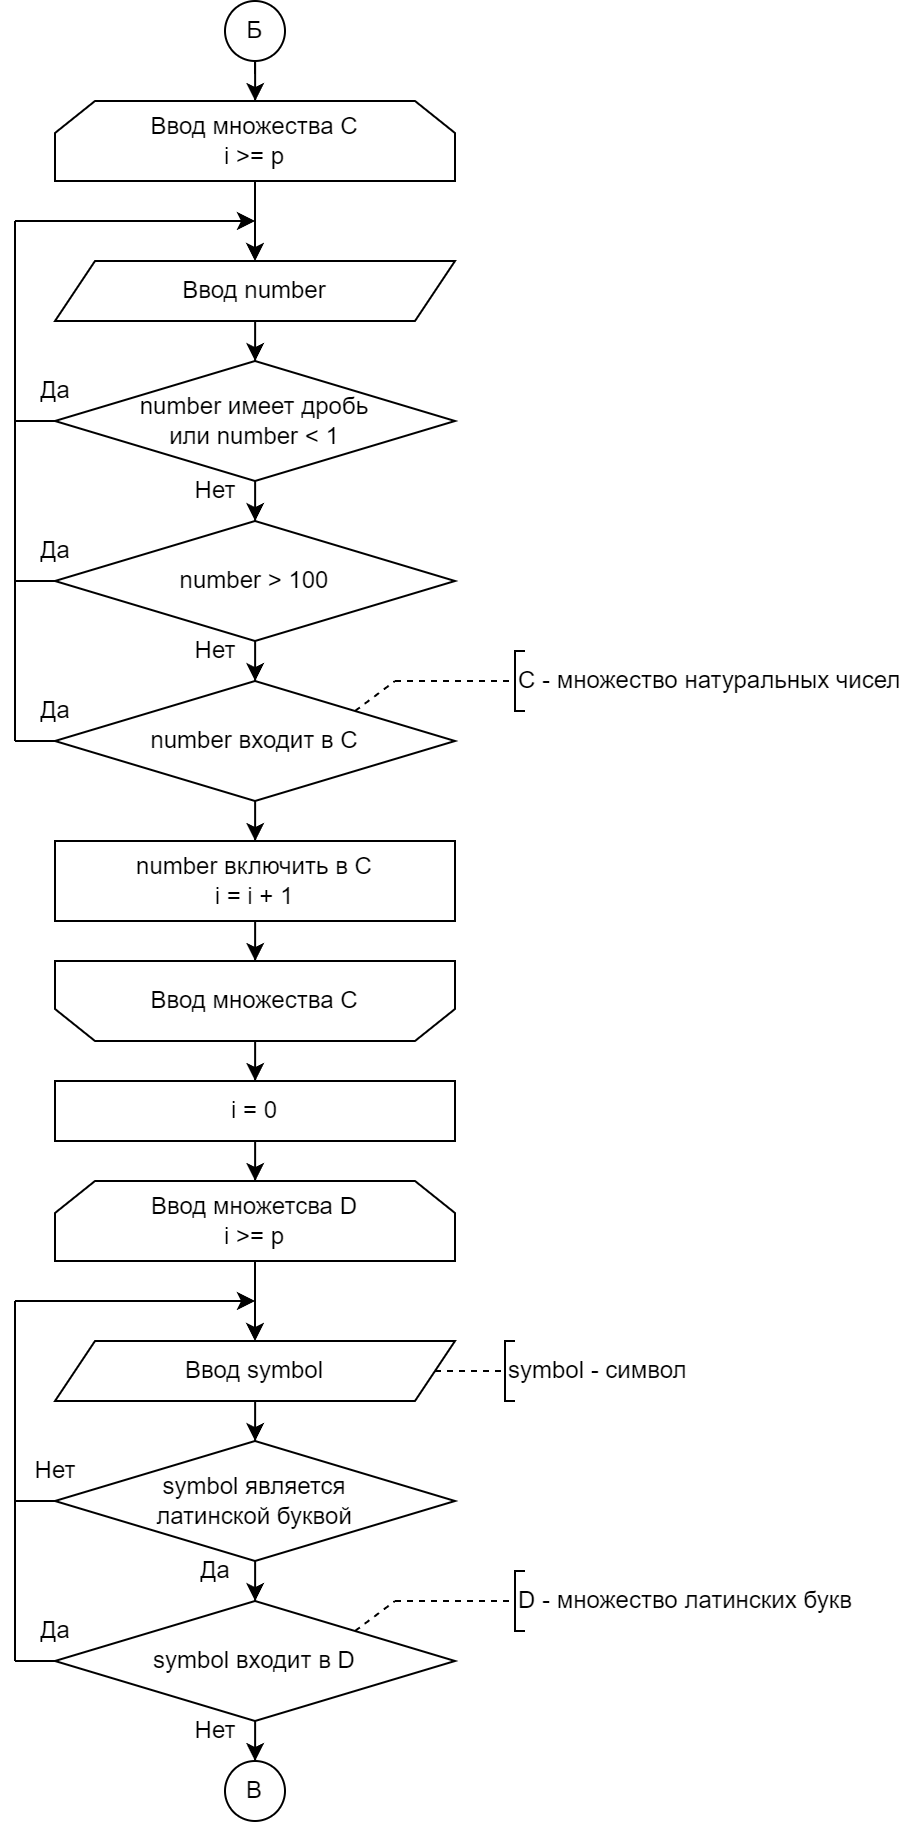
\includegraphics[width=0.58\linewidth]{images/s-3}
  \end{figure}
  \begin{center}
    Рисунок 3 – Продолжение схемы алгоритма программы
  \end{center}
  
  \pagebreak
  \begin{figure}[h]
    \centering
    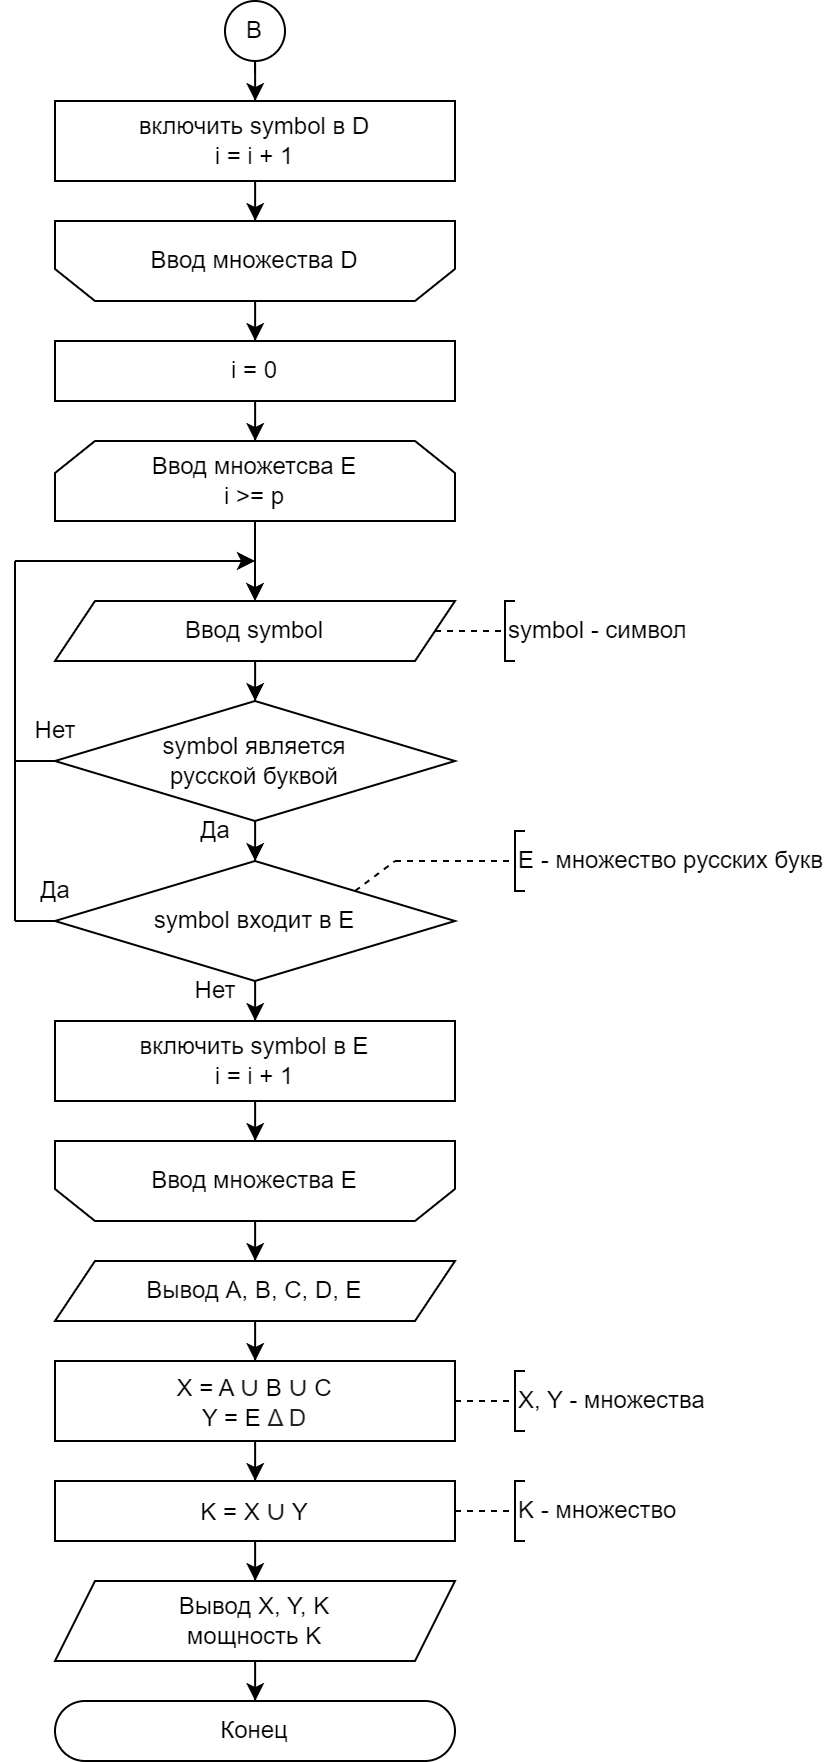
\includegraphics[width=0.55\linewidth]{images/s-4}
  \end{figure}
  \begin{center}
    Рисунок 4 – Продолжение схемы алгоритма программы
  \end{center}
  
  \pagebreak
  При разработке реализована программа, исходный код которой представлен ниже.
  \begin{Verbatim}[tabsize=2]
program solution;
var
  A, B, C, D, E: set of string;
  bf: string;
  p, i: byte;
  error: boolean;
  number: real;
  numerator, denominator: integer;
  symbol: char;
begin
  error := true;
  repeat
    write('Введите мощность множеств (не более 10): ');
    try
      readln(p);
      error := false;
    except
      writeln('Неверный формат ввода');
    end;
  until (p >= 1) and (p <= 10) and not error;
  write('Введите множество (A) действительных чисел (-100 - 100): ');
  i := 0;
  while i < p do
  begin
    try
      read(number);
      if (number > 100) or (number < -100) then
      begin
        writeln('Выход за пределы значения числа');
        continue;
      end;
      bf := FloatToStr(number);
      if bf in A then
      begin
        writeln('Число ', bf, ' уже входит в множество');
        continue;
      end;
      include(A, bf);
      i := i + 1;
    except
      writeln('Неверный формат ввода');
    end;
  end;
  readln();
  writeln('Введите множество (B) рациональых чисел: ');
  i := 0;
  while i < p do
  begin
    try
      write('Введите числитель: ');
      readln(numerator);
      repeat
        write('Введите знаменатель: ');
        read(denominator);
        if denominator < 1 then
          writeln('Знаменатель не может быть меньше 1');
      until denominator > 0;
      number := int(numerator) / int(denominator);
      bf := FloatToStr(number);
      if bf in B then
      begin
        writeln('Число ', bf, ' уже входит в множество');
        continue;
      end;
      include(B, bf);
      i := i + 1;
    except
      writeln('Неверный формат ввода');
    end;
  end;
  readln();
  write('Введите множество (С) натуральных чисел (1 - 100): ');
  i := 0;
  while i < p do
  begin
    try
      read(number);
      if (frac(number) <> 0) or (number < 1) then
      begin
        writeln('Число ', number, ' не является натуральным');
        continue;
      end;
      if number > 100 then
      begin
        writeln('Превышен предел значения числа');
        continue;
      end;
      bf := FloatToStr(number);
      if bf in C then
      begin
        writeln('Число ', bf, ' уже входит в множество');
        continue;
      end;
      include(C, bf);
      i := i + 1;
    except
      writeln('Неверный формат ввода');
    end;
  end;
  readln();
  write('Введите множество (D) латинских букв: ');
  i := 0;
  while i < p do
  begin
    try
      read(symbol);
      if (ord(symbol) = 32) or (ord(symbol) = 10) or (ord(symbol) = 13) then continue;
      if ((ord(symbol) >= 65) and (ord(symbol) <= 90)) or 
      ((ord(symbol) >= 97) and (ord(symbol) <= 122)) then
        bf := symbol
      else
      begin
        writeln('Буква ', symbol, ' не является латинской');
        continue;
      end;
      if bf in D then
      begin
        writeln('Буква ', bf, ' уже входит в множество');
        continue;
      end;
      include(D, bf);
      i := i + 1;
    except
      writeln('Неверный формат ввода');
    end;
  end; readln();
  write('Введите множество (E) русских букв: ');
  i := 0;
  while i < p do
  begin
    try
      read(symbol);
      if (ord(symbol) = 32) or (ord(symbol) = 10) or (ord(symbol) = 13) then continue;
      if (ord(symbol) >= 1040) and (ord(symbol) <= 1103) then
        bf := symbol
      else
      begin
        writeln('Буква ', symbol, ' не является латинской');
        continue;
      end;
      if bf in E then
      begin
        writeln('Буква ', bf, ' уже входит в множество');
        continue;
      end;
      include(E, bf);
      i := i + 1;
    except
      writeln('Неверный формат ввода');
    end;
  end;
  readln();
  writeln('A = ', A, ' ');
  writeln('B = ', B, ' ');
  writeln('C = ', C);
  writeln('D = ', D, ' ');
  writeln('E = ', E);
  writeln('X = A * B * C = ', A * B * C);
  writeln('Y = (E + D) - (E * D) = ', (E + D) - (E * D));
  writeln('K = X + Y = ', (A * B * C) + ((E + D) - (E * D)));
  writeln('Мощность множества K = ', ((A * B * C) + ((E + D) - (E * D))).count);
  readln;
end.
  \end{Verbatim}
  
  Экранная форма программы в виде консольного приложения представлена на рисунке 5.
  \begin{figure}[h]
    \centering
    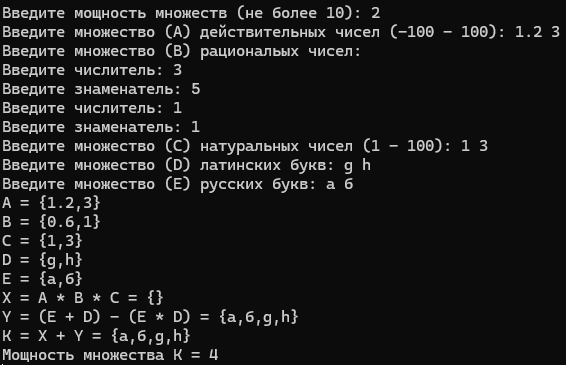
\includegraphics[width=0.8\linewidth]{images/screen}
  \end{figure}
  \begin{center}
    Рисунок 5 – Консольный интерфейс программы
  \end{center}
  
  \section*{Вывод}
  В процессе выполнения лабораторной работы, при решении предложенных задач, изучены операции над множествами и реализованы такие операции как пересечение, симметричная разность, мощность множества. Для решения реализована программа на языке Паскаль, представляющая из себя консольный интерфейс, которая выводит результат решения задач.

\end{document}